% mnras_template.tex
%
% LaTeX template for creating an MNRAS paper
%
% v3.0 released 14 May 2015
% (version numbers match those of mnras.cls)
%
% Copyright (C) Royal Astronomical Society 2015
% Authors:
% Keith T. Smith (Royal Astronomical Society)

% Change log
%
% v3.0 May 2015
%    Renamed to match the new package name
%    Version number matches mnras.cls
%    A few minor tweaks to wording
% v1.0 September 2013
%    Beta testing only - never publicly released
%    First version: a simple (ish) template for creating an MNRAS paper

%%%%%%%%%%%%%%%%%%%%%%%%%%%%%%%%%%%%%%%%%%%%%%%%%%
% Basic setup. Most papers should leave these options alone.
\documentclass[a4paper,fleqn,usenatbib]{mnras}

% MNRAS is set in Times font. If you don't have this installed (most LaTeX
% installations will be fine) or prefer the old Computer Modern fonts, comment
% out the following line
\usepackage{newtxtext,newtxmath}
% Depending on your LaTeX fonts installation, you might get better results with one of these:
%\usepackage{mathptmx}
%\usepackage{txfonts}

% Use vector fonts, so it zooms properly in on-screen viewing software
% Don't change these lines unless you know what you are doing
\usepackage[T1]{fontenc}
\usepackage{ae,aecompl}


%%%%% AUTHORS - PLACE YOUR OWN PACKAGES HERE %%%%%

% Only include extra packages if you really need them. Common packages are:
\usepackage{graphicx}	% Including figure files
\usepackage{amsmath}	% Advanced maths commands
\usepackage{amssymb}	% Extra maths symbols
\usepackage{hyperref}

%%%%%%%%%%%%%%%%%%%%%%%%%%%%%%%%%%%%%%%%%%%%%%%%%%

%%%%% AUTHORS - PLACE YOUR OWN COMMANDS HERE %%%%%

% Please keep new commands to a minimum, and use \newcommand not \def to avoid
% overwriting existing commands. Example:
%\newcommand{\pcm}{\,cm$^{-2}$}	% per cm-squared

% Definitions
\defcitealias{Mertens2018}{M18}
\defcitealias{Mertens2020}{M20}
\defcitealias{Gosh2020}{G20}
\newcommand{\nsk}[1]{{\color{blue} \textbf{[NSK:  #1]}}}
\def\para{\parallel}
\def\d{\boldsymbol{d}}
\def\D{\boldsymbol{D}}
\def\e{\boldsymbol{e}}
\def\E{\boldsymbol{E}}
\def\f{\boldsymbol{f}}
\def\F{\boldsymbol{F}}
\def\H{\boldsymbol{H}}
\def\r{\boldsymbol{r}}
\def\R{\boldsymbol{R}}
\def\n{\boldsymbol{n}}
\def\N{\boldsymbol{N}}
\def\u{\boldsymbol{u}}
\def\k{\boldsymbol{k}}
\def\T{\boldsymbol{T}}
\def\x{\boldsymbol{x}}
\def\g{\boldsymbol{g}}
\def\q{\boldsymbol{q}}
\def\p{\boldsymbol{p}}
\def\Q{\boldsymbol{Q}}
\def\w{\boldsymbol{w}}
\def\m{\boldsymbol{m}}
\def\M{\boldsymbol{M}}
\def\C{\boldsymbol{C}}
\def\W{\boldsymbol{W}}
\def\V{\boldsymbol{V}}
\def\Cfg{\boldsymbol{C}_{\rm fg}}
\def\Cto{\boldsymbol{C}_{\rm 21}}
\def\Cn{\boldsymbol{C}_{\rm n}}
\def\Cip{\boldsymbol{C}_{\rm ip}}
\def\dip{\boldsymbol{d}_{\rm ip}}
\def\I{\boldsymbol{I}}
\def\Cov{{\rm Cov}}
\def\Exp{{\rm E}}
\def\bSigma{\boldsymbol{\Sigma}}
\def\bnu{\boldsymbol{\nu}}
\def\btheta{\boldsymbol{\theta}}
\def\K{\boldsymbol{K}}
\def\bk{\boldsymbol{k}}
\def\Kto{K_{\rm 21}}
\def\Kfg{K_{\rm fg}}
\def\Kn{K_{\rm n}}
\def\Kip{K_{\rm ip}}
\def\sigmafg{\sigma_{\rm fg}}
\def\ellfg{\ell_{\rm fg}}
\def\sigman{\sigma_{\rm n}}
\def\sigmato{\sigma_{\rm 21}}
\def\ellto{\ell_{\rm 21}}
\def\A{\boldsymbol{A}}
\def\B{\boldsymbol{B}}
\def\U{\boldsymbol{U}}
\def\S{\boldsymbol{S}}
\def\V{\boldsymbol{V}}
\def\kpara{k_{\parallel}}
\def\kperp{k_{\perp}}
\def\tr{{\rm tr}}

%%%%%%%%%%%%%%%%%%%%%%%%%%%%%%%%%%%%%%%%%%%%%%%%%%

%%%%%%%%%%%%%%%%%%% TITLE PAGE %%%%%%%%%%%%%%%%%%%

% Title of the paper, and the short title which is used in the headers.
% Keep the title short and informative.
\title[Joint Gaussian Process Foreground Subtraction and Power Spectrum Estimation]
{Joint Gaussian Process Foreground Subtraction and Power Spectrum Estimation for 21\,cm Cosmology}

% The list of authors, and the short list which is used in the headers.
% If you need two or more lines of authors, add an extra line using \newauthor
\author[N. S. Kern \& A. C. Liu]{
Nicholas S. Kern$^{1}$\thanks{E-mail: nkern@berkeley.edu},
Adrian C. Liu$^{2}$
\\
$^{1}$Department of Astronomy, University of California, Berkeley, CA, USA\\
$^{2}$Department of Physics and McGill Space Institute, McGill University, 3600 University Street, Montreal, QC H3A 2T8, Canada
}

% These dates will be filled out by the publisher
\date{Accepted XXX. Received YYY; in original form ZZZ}

% Enter the current year, for the copyright statements etc.
\pubyear{2015}

% Don't change these lines
\begin{document}
\label{firstpage}
\pagerange{\pageref{firstpage}--\pageref{lastpage}}
\maketitle

% Abstract of the paper
\begin{abstract}
One of the key challenges in enabling the science potential of 21\,cm intensity mapping experiments is the separation of bright astrophysical foreground contamination from the underlying cosmological signal.
Surmounting this challenge will unlock major sensitivity boosts for future 21\,cm experiments targeting both the pre and post reionization epoch, and will also enable for the cross-correlation of the 21\,cm signal with other probes of large scale structure.
Foreground signal separation is generally most challenging at low spatial Fourier $k$ modes, where foreground contamination is the strongest.
Recent works have claimed that a Bayesian approach to data modeling using Gaussian process regression (GPR) can robustly perform this separation and may enable a 21\,cm detection at these low $k$ modes.
We investigate these claims by casting GPR foreground subtraction into the quadratic estimator formalism, thereby putting its statistical properties on stronger theoretical footing.
Specifically, we find that without careful treatment of the low $k$ window functions, GPR foreground subtraction can significantly bias the recovered power spectrum.
Furthermore we study the impact of inaccurate covariance models in the data modeling process, showing that it too can lead to biases in the recovered power spectrum.
We propose an approach for handling these effects when applying GPR data modeling to 21\,cm data analysis pipelines.
Incidentally, we find that under certain conditions GPR foreground subtraction is identical to the optimal inverse covariance quadratic estimator widely studied for power spectrum estimation.
\end{abstract}

% Select between one and six entries from the list of approved keywords.
% Don't make up new ones.
\begin{keywords}
keyword1 -- keyword2 -- keyword3
\end{keywords}

%%%%%%%%%%%%%%%%%%%%%%%%%%%%%%%%%%%%%%%%%%%%%%%%%%

%%%%%%%%%%%%%%%%% BODY OF PAPER %%%%%%%%%%%%%%%%%%

\section{Introduction}
\label{sec:intro}

Foreground separation for 21\,cm cosmology has the potential to significantly increase the sensitivity of current and future cosmological datasets.
Many methods have been developed for doing this, some show more promise than others.
Recently, Gaussian process based data modeling approaches have been proposed as a promising technique, and have become more widely used in real analysis pipelines.
In this work, we put Gaussian process based foreground subtraction on stronger theoretical footing by propagating its statistical properties into the quadratic estimator formalism, thus allowing us to derive the power spectrum band power covariances and window functions of this method for the first time.

Novel components of this work are...


%%%%%%%%%%%%%%%%%%%%%%%%%%%%%%%%%%%%%%%%%%
%%%%%%%%%%%%%%%%% Formalism %%%%%%%%%%%%%%%%%%%
%%%%%%%%%%%%%%%%%%%%%%%%%%%%%%%%%%%%%%%%%%
\section{Data Modeling Formalism}
\label{sec:formalism}

In this section we describe the various components of the data vector for 21\,cm cosmology experiments, outlining how astrophysical foregrounds, the cosmological signal, and various instrumental contaminants appear in the data.
We then describe the formalism for Bayesian modeling of these components using a Gaussian process.
For more details on interferometric measurements see \citet{Hamaker1996, Smirnov2011}.
Also, for a comprehensive overview of Gaussian process modeling we refer the reader to \citet{Rasmussen2006}.


\subsection{Radio Inteferometric Measurements}
\label{sec:rime}

The fundamental observable for a radio interferometer is the interferometric visibility, $V_{jk}$, formed by the voltage correlation of two antennas $j$ and $k$, which is related to the specific intensity of the sky temperature via the measurement equation:
\begin{align}
\label{eq:me}
V_{jk}(\nu) = \int_{4\pi}d\Omega\ A(\hat{s}, \nu)I(\hat{s},\nu)e^{2\pi i\boldsymbol{b}_{jk}\cdot\boldsymbol{\hat{s}}\nu/c},
\end{align}
where $A$ is the direction and frequency dependent primary beam response of the antennas, $I$ is the sky temperature field, and the exponential holds the interferometric fringe term \citep{Thompson}.
Given a model of the sky and of the antenna primary beam response, the visibility is a complex-valued quantity that is uniquely specified by the baseline vector, $\boldsymbol{b}_{jk}$.
Assuming the sky is dominated by a collection of point sources allows us to drop the integral in place of a discrete sum for each point source's flux density.
We can therefore write \autoref{eq:me} as
\begin{align}
\label{eq:me2}
V_{jk}(\nu) = \sum_lA_l(\nu)S_l(\nu)e^{2\pi i\tau_{jk,l}\nu},
\end{align}
where $l$ indexes each point source on the sky, $S$ is their flux density, and we have re-written the exponential argument in terms of the relative delay lag of the point source's wavefront with respect to the baseline vector, $\tau_{jk} = \boldsymbol{b}_{jk}\cdot\hat{s}/c$.
Written this way, we see from \autoref{eq:me2} that the visibility response to a single point source as a function of frequency is just a Fourier term ($\tau$ being the Fourier dual to $\nu$) enveloped by the amplitude of the primary beam and the intrinsic source brightness.
This tells us two things about the frequency dependence of the visibility: 1. that for bandwidths larger than $1/\tau_{jk}$ the visibility is a mean-zero process, and 2. that the amplitude of this process is frequency dependent--in other words it is non-stationary.

The form of \autoref{eq:me2} also tells us something about the amount of \emph{spectral structure} that is contained within the visibility.
Low-frequency radio foreground emission, either from the Milky Way galactic plane or from individual radio galaxy point sources, is generally regarded to be spectrally smooth, as it is thought to be predominately generated by non-thermal synchrotron emission with a characteristic spectral slope of $\nu^{-2}$ \citep{Condon}.
If we were to take the Fourier transform of their continuum spectra, then, we would find that most of their power would be confined to small delay ($\tau$) Fourier modes.
However, the act of the Fourier term $e^{2\pi i\tau_{jk}\nu}$ in \autoref{eq:me2} can be thought of as an overall phasor that boosts the smooth spectrum foreground to large delays of $\pm\tau_{jk}$.
This is what undergirds the statement that a radio interferometer is inherently chromatic, and is the origin of the instrument-induced ``foreground wedge,'' which causes smooth spectrum foregrounds to gain additional structure in the visibilities \citep{Datta2010, Morales2012}.

Recall that $\tau_{jk} = \boldsymbol{b}_{jk}\hat{s}/c = |b_{jk}|\cos(\theta)/c$ where $\theta$ is the angle between $\boldsymbol{b}_{jk}$ and $\hat{s}$.
This tells us that the maximum delay a foreground source can be boosted to is $\tau_{jk}^{\rm horizon} = b_{jk}\cos(0)/c$, which coincides with a foreground source incident from the baseline horizon.
For any realistic telescope, point source and diffuse foregrounds are incident from all angles on the sky but are more suppressed by the primary beam when incident closer to the horizon.
Thus, the aggregate observed spectral structure of foregrounds in the visibility in the delay domain is generally something roughly like a Gaussian profile centered at $\tau=0$ seconds with power extending out to $\tau=\pm\tau_{jk}^{\rm horizon}$ \citep{Parsons2012b}.
This is an important feature that shapes how we discuss the data.
When we use the term ``within the wedge,'' we mean all delays in the visibility data that are foreground dominated (generally $|\tau| < \tau^{\rm horizon}$), whereas ``outside the wedge'' the data are either noise or EoR dominated (or, as is often the case, dominated by some other systematic).
To model foreground structure in the visibilities, one seeks to construct a model of smoothly varying functions that can fit arbitrary (non-parametric) spectral structure that is compact in delay space down to a frequency length scale of $\ell_{jk} = 1/\tau_{jk}$ Hz.

Unfortunately this is not the entire picture for realistic 21\,cm radio experiments.
There are in practice other terms that cause $S(\nu)$ to pick up extra sources of spectral structure in the visibilities.
From \autoref{eq:me2} we can already see one of them, which is the frequency dependence of the primary beam.
Near the pointing center we expect the derivative of the beam with respect to frequency to be small, but further away this derivative can spike, especially near primary beam nulls, which causes off-axis foreground emission to pick up even more spectral structure.
Yet another common term is the gain response of the instrument, which can have an arbitrary amount of structure depending on the array configuration (e.g. the position of the feed) and its hardware (e.g. performance of RF signal chain, bandpass, etc).
The (direction independent) instrumental gain is imparted to the data in the visibility domain, and relates the \emph{measured} visibility to the true visibility as
\begin{align}
V_{jk}^{\rm measured}(\nu) = V_{jk}(\nu)g_j(\nu)g_k(\nu)^\ast,
\end{align}
where $g_j$ and $g_k$ are the complex gains for antennas $j$ and $k$.
Gain calibration attempts to mitigate this by solving for and inverting the gain response of each antenna, but this is still an active area of research as it has yet to be shown that this can actually be done for realistic experiments to the precision required for EoR science.
For example, recent works have shown that calibration errors from a number of different calibration techniques can easily exceed the underlying 21\,cm signal in the data, thus prohibiting its detection in the power spectrum \citep{Barry2016, Ewall-Wice2017, Dillon2017, Orosz2018, Byrne2019, Jospeh2019, Kern2020b}.


\subsection{Gaussian Process Regression}
\label{sec:gpr}

Here we review Gaussian process regression, drawing from \citet{Rasmussen2006} for the general formalism, and \citet{Mertens2018} for applications to 21\,cm foreground subtraction.
\nsk{need to merge scipy w/ QE class}
In this work we use the \texttt{scipy}\footnote{scipy} package's optimized implementation of the Gaussian process predictive equation \autoref{eq:gp_conditional}, which is derived from \citet{Rasmussen2006}.

Let our dependent data be described as a column vector, $\d$, containing the complex visibility for a particular baseline at each frequency, and let the column vector $\boldsymbol{\nu}$ hold the frequencies of the data, such that
\begin{align}
\label{eq:dvec}
\d = \begin{bmatrix}d_1\\ d_2\\ \vdots\\ d_n\end{bmatrix}; \boldsymbol{\nu} = \begin{bmatrix}\nu_1\\ \nu_2\\ \vdots\\ \nu_n\end{bmatrix}.
\end{align}
Multiple observations (in radio terminology, integrations) can be incorporated by expanding our data vector as an $n\times m$ matrix, where $m$ is the number of integrations in the data.
Multiple baselines can similarly be accounted for by appending along this axis.
Nominally, our data vector for a particular baseline consists of the measured foreground ($f$), EoR signal ($e$), and thermal noise ($n$),
\begin{align}
\label{eq:data_vec}
\d = \f + \e + \n,
\end{align}
which are statistically uncorrelated.
Thus the covariance of the data is given by
\begin{align}
\label{eq:data_cov}
\C = \langle\d\d^T\rangle = \Cfg + \Cto + \Cn,
\end{align}
where $\langle\rangle$ denotes an ensemble average.
Assuming our data vector is Gaussian distributed, we can model its probability distribution as
\begin{align}
\d\sim\mathcal{N}\left(m(\bnu), K(\bnu, \bnu)\right),
\end{align}
where $m$ is an underlying mean function of our model and $K$ is its covariance function (or kernel).
In other words, we assume that our data vector is a discrete realization of a class of continuous fields drawn from a Gaussian distribution in function space, or a Gaussian process.
Given our conclusions from \autoref{sec:rime} we assume the mean function of our GP to be zero.

Given our measurements, $\d$, we can write down the joint distribution of the Gaussian process at a series of other points in space $\bnu^\prime$ as
\begin{align}
\label{eq:joint_gp}
\begin{bmatrix}\d \\ \d^\prime\end{bmatrix} \sim \mathcal{N}\left(\begin{bmatrix}0\\ 0\end{bmatrix},
\begin{bmatrix}K(\bnu,\bnu) & K(\bnu,\bnu^\prime)\\K(\bnu^\prime, \bnu) & K(\bnu^\prime,\bnu^\prime)\end{bmatrix}\right).
\end{align}
In general GP applications, we are usually interested in learning something about the Gaussian process at the new points in space given our knowledge of the measured data vector.
To get this, we condition the Gaussian process on our measurements, yielding a probability distribution on $\d^\prime$
\begin{align}
\d^\prime|\d \sim \mathcal{N}\left(\Exp[\d^\prime], \Cov[\d^\prime]\right),
\end{align}
where $\Exp[]$ is the expectation value, $\Cov[]$ is the covariance, and
\begin{align}
\label{eq:gp_conditional}
\Exp[\d^\prime] &= K(\nu^\prime,\nu)K(\nu,\nu)^{-1}\d \\
\Cov[\d^\prime] &= K(\nu^\prime,\nu^\prime) - K(\nu^\prime, \nu)K(\nu, \nu)^{-1}K(\nu, \nu^\prime).
\end{align}

For the case of foreground modeling in interferometric visibility data, what we want to extract is an estimate of our foreground model $f^\prime$ given our measurements $d$ (generally at the same frequencies $\bnu$, but we revisit this in \autoref{sec:contaminants}).
To do this, we pick a model for the covariance of each term in the data, $K = \Kfg + \Kto + \Kn$, and plug them into \autoref{eq:joint_gp}.
This gives us the joint distribution on our data and estimated foreground model,
\begin{align}
\begin{bmatrix}\d \\ \f^\prime\end{bmatrix} \sim \mathcal{N}\left(\begin{bmatrix}0\\ 0\end{bmatrix},
\begin{bmatrix}\Kfg+\Kto+\Kn & \Kfg\\ \Kfg & \Kfg\end{bmatrix}\right),
\end{align}
where the off-diagonal terms in the joint density covariance matrix simplify to $\Kfg$ because the foreground vector is the only data term that is correlated between $\f^\prime$ and $\d$.
Using \autoref{eq:gp_conditional}, we then find that
\begin{align}
\label{eq:fg_conditional}
\Exp[\f^\prime] &= \Kfg [\Kfg+\Kto+\Kn]^{-1}\d \\
\label{eq:fg_cov_conditional}
\Cov[\f^\prime] &= \Kfg - \Kfg[\Kfg+\Kto+\Kn]^{-1}\Kfg.
\end{align}
For foreground removal applications, we are interested in forming the data residual vector,
\begin{align}
\label{eq:res}
\r = \d - \Exp[\f^\prime],
\end{align}
which we hope subtracts the foregrounds and reveals the 21\,cm signal.
In this work, we will use the term ``residual'' to mean exclusively the vector $\r$.
Note that there is a difference between the covariance kernel we choose to model a specific term in the data vector, (e.g. $K_{\rm fg}$) and the actual covariance of that term (e.g. $\Cfg$), the latter of which is generally never known exactly.
Ideally we want these to be as close as possible, but they are not by construction equivalent.

In this work, we model the foregrounds with a radial basis function (or a squared exponential kernel),
\begin{align}
\label{label:fg_kernel}
\Kfg(\nu, \nu^\prime) = \sigmafg^2\exp\left(-\frac{(\nu-\nu^\prime)^2}{2\ellfg^2}\right),
\end{align}
which produces very smoothly varying functions.
This is motivated by the fact that foregrounds, although imparted with some spectral structure by the instrument, are thought to be spectrally smooth.
The function hyperparameters, the overall variance $\sigmafg^2$ and the length scale $\ellfg$, are tunable parameters of the kernel.
The length scale can be thought of as the characteristic size scale a random field drawn from such a covariance fluctuates at.
Recall we outlined the rough amount of foreground spectral structure we expect to see in a visibility depending on its baseline length and what frequency scale that translates to (\autoref{sec:rime}).
Therefore, we already have a good, physically motivated guess for what these hyperparameters should be, although we will return to how we actually refine these estimates in a data-driven manner.
\citetalias{Mertens2018} go one step further and break down the foreground covariance into two separable covariances, one for modeling broad scale foreground fluctuations and one for modeling intermediate scale fluctuations.
In this work, we stick with the single-kernel option for simplicity.\footnote{We also did not find noticeable improvement in our simulations using two kernels for the foreground covariance.}

The 21\,cm signal is expected to be much more spectrally variant and is not well modeled by a radial basis function.
Instead, similar to \citetalias{Mertens2018}, we use an exponential function,
\begin{align}
\label{label:eor_kernel}
\Kto(\nu, \nu^\prime) = \sigmato^2\exp\left(-\frac{|\nu-\nu^\prime|}{\ellto}\right),
\end{align}
which has far less covariance between largely separated frequencies, and therefore models quick spectral features better.
An exponential distribution seems to match some of the signal covariances derived from large scale simulations of $\delta T_{21}$ decently well;
however, something we will return to is what happens when this assumption breaks down.
Lastly, we use a simple scalar matrix to model the noise, which is uncorrelated from channel to channel,
\begin{align}
\Kn(\nu, \nu^\prime) = \sigman^2\delta_{\nu\nu^\prime},
\end{align}
where $\delta_{\nu\nu^\prime}$ is the Kronecker delta, which is one if $\nu=\nu^\prime$ and zero otherwise..

Note that we've chosen to model our covariance functions as stationary: in other words, they are independent of where in $\nu$ they are evaluated and only depend on $\nu-\nu^\prime$.
However, this is not strictly true for some of the terms in our data, as we saw in \autoref{sec:rime}.
For example, we know that low-frequency foregrounds become brighter at lower frequencies, following a $\nu^{-2}$ power law (Haslam).
Similarly, thermal noise is also non-stationary, rising at low frequencies due to the increase in sky noise temperature.
For transit telescopes like HERA, these terms are also \emph{time dependent}, as the optimal foreground amplitude and length scale and noise amplitude will change depending on what sources are in the primary beam.
For this work, we concern ourself with a fairly narrow spectral window and only consider a single time integration, so these are largely second order effects.
However, for wide-band and multi-integration foreground modeling, these effects will likely need to be taken into account.

\subsubsection{Hyperparameter Optimization}
\label{sec:optimization}
The kernel hyperparameters can be selected using Bayesian model selection to determine the values that best fit the data.
This is done by maximizing the marginal likelihood, or the Bayesian evidence, which is the integral of the data likelihood times our prior on the data,
\begin{align}
p(\d|\bnu, \btheta) = \int \mathcal{L}(\d|\g,\bnu,\btheta)p(\g|\bnu)d\g,
\end{align}
where $\g$ is another vector spanning the space of our data and $\btheta$ is a vector containing our kernel hyperparameters.
This Gaussian integral can be done analytically, and is given up to a constant as
\begin{align}
\label{eq:ml}
\log p(\d|\bnu,\btheta) \propto -\frac{1}{2}\d^TK(\bnu,\bnu|\btheta)^{-1}\d - \frac{1}{2}\log{\rm det}|K(\bnu,\bnu|\btheta)|,
\end{align}
where recall $K$ is the full covariance function of our data \citep{Rasmussen2006}.
The posterior distribution on our hyperparameters is then proportional to the log marginal likelihood plus the log prior: $\log p(\d|\bnu,\btheta) + \log p(\btheta)$.
We use a Markov Chain Monte Carlo (MCMC) algorithm to explore the joint hyperparameter posterior distribution and determine the maximum a posteriori (MAP) vector $\hat{\btheta}$.
This uses the affine-invariant sampler of \citet{Goodman} found in the \texttt{emcee}\footnote{emcee} package \citep{Foreman-Mackey}.

\section{GPR Foreground Subtraction in the Quadratic Estimator Framework}
\label{sec:gprfs}

In this section we outline how GPR foreground subtraction can be incorporated into the quadratic estimator formalism.
We start by giving a brief review of quadratic estimators, and then demonstrate GPR-FS, or a GPR foreground subtracted quadratic estimator.
Principally, we show that this is closely related to the inverse covariance estimator outlined in \citet{Liu2011}.
We also discuss some variations to GPR-FS that allow for estimation of the foreground component (which is often useful for null testing and data quality management), in addition to handling the issue of missing data (e.g. due to RFI flags).
Lastly, most of the results of this section hinges on the assumption that the exact covariance of the data is known a priori.
Previous works have shown that one can either estimate the covariance from the data directly (T97, Seljak, Switzer?, Dillon2014), or one can adopt a fiducial covariance and iterate (Padmanabhan).
However, this is particularly tricky for EoR studies, where the EoR 21\,cm power spectrum is greatly unconstrained, and recent examples of empirically estimated covariances have led to signal loss \citep{Cheng2018}.
We discuss some of the potential pitfalls from this problem for detection of the EoR power spectrum at low $k$.

\subsection{Quadratic Estimators of the Power Spectrum}
\label{sec:qe}

The 21\,cm power spectrum is the square of the three dimensional Fourier transform of the temperature,
\begin{align}
\langle\widetilde{\T}(\boldsymbol{k})\widetilde{\T}^\ast(\boldsymbol{k}^\prime)\rangle = P(k)\delta(\boldsymbol{k}-\boldsymbol{k}^\prime),
\end{align}
where $\widetilde{\T}$ is the Fourier transformed temperature field, and $\delta$ is the Dirac-delta function.
Noting that the interferometric visibilities are simply the transverse Fourier transform of the sky (under the flat sky approximation), an estimate of the power spectrum can be made by directly Fourier transforming the visibilities across frequency into the delay domain $\tau$, known as the delay spectrum estimator \citep{Parsons2012a, Liu2014a}.
Due to the inherent chromaticity of the interferometer (i.e. it samples different spatial Fourier modes as a function of frequency), the visibility delay domain is not an exact mapping to the line-of-sight spatial Fourier domain, but for short baselines this is a fairly good approximation \citep{Parsons2012a}.
In this case, the power spectrum is defined as
\begin{align}
\label{eq:dspec}
P(k_\perp, k_\para) = \frac{X^2Y}{\Omega_pB}\langle\widetilde{V}(\boldsymbol{b}/\lambda, \tau)\widetilde{V}^\ast(\boldsymbol{b}/\lambda, \tau)\rangle,
\end{align}
where $X$ and $Y$ are scalars mapping angles on the sky to transverse cosmological distances and frequencies to line-of-sight cosmological distances, $\Omega_p$ is the integral of the primary beam and $B$ is the frequency bandwidth in the Fourier transform.
The cosmological wavevectors are related to the ``telescope units'' via
\begin{align}
\label{eq:kvecs}
k_\perp &= \frac{2\pi\tau}{X} \\
k_\para  &= \frac{2\pi}{Y}\frac{b}{\lambda},
\end{align}
where $X = c(1+z)^2\nu_{21}^{-1}H(z)^{-1}$, $Y=D(z)$, $\nu_{21}=1.420$ GHz, $H(z)$ is the Hubble parameter, $\lambda$ is the average observing wavelength, and $D(z)$ is the transverse comoving distance \citep{Parsons2014}.
In this work we adopt a $\Lambda$CDM cosmology with parameters derived from the Planck 2015 analysis \citep{Planck2016}, specifically $\Omega_\Lambda$=0.6844, $\Omega_b$=0.04911, $\Omega_c$=0.26442, and $H_0$=67.27 km/s/Mpc.

To be more statistically rigorous, we can cast the delay spectrum technique into the quadratic estimator framework \citep{Hamilton1997, Tegmark1997, Liu2014a}.
We start by approximating the continuous power spectrum as a piecewise function in sufficiently narrow bins in $k$.
The $\alpha$ bin's amplitude, $p_\alpha$, is referred to as its band power, and its reconstruction from the data is the ultimate goal of our estimator.
Fundamentally, we assume that the covariance of the data in frequency space can be related to the band powers as
\begin{align}
\label{eq:bandpowers}
\C = \N + \Cfg + \sum_\alpha p_\alpha \C_{,\alpha},
\end{align}
where $\N$ is our noise covariance, $\Cfg$ is our foreground covariance, $p_\alpha$ is our EoR power spectrum band powers, and $\C_{,\alpha} = \partial\C/\partial p_\alpha$ is the derivative of the covariance matrix with respect to the band powers (the response matrix).
A quadratic estimate of the band powers can be formed from our data vectors as
\begin{align}
\label{eq:qe}
\hat{p}_\alpha = \d^\dagger\E_\alpha\d - b_\alpha,
\end{align}
where recall $\d$ is our data vector, $\hat{p}_\alpha$ is our estimate of the $\alpha$ band power, $\E$ is a family of matrices to-be-described, and $b_\alpha$ is an overall bias term.
Taking the expectation value of \autoref{eq:qe} and substituting in \autoref{eq:bandpowers}, we find that 
\begin{align}
\label{eq:window_funcs}
\langle\hat{p}_\alpha\rangle = \sum_\beta\tr[\C_{,\beta}\E_\alpha]p_{\beta} + \tr[(\N + \Cfg)\E_\alpha] - b_\alpha.
\end{align}
\autoref{eq:window_funcs} tells us that for our estimator to be unbiased we set $b_\alpha = \tr[(\N+\Cfg)\E_\alpha]$.
Furthermore, it shows us that the estimated band powers $\hat{p}_\alpha$ are a linear combination of the true band powers $p_\alpha$ dictated by a transfer matrix, which we will denote as $\W$, commonly known as the \emph{window function}: $\hat{\p} = \W\p$.
The covariance of our band powers subject to the covariance of our input data can be written as
\begin{align}
\label{eq:qe_C}
\Sigma_{\alpha\beta} = \langle \hat{p}_\alpha\hat{p}_\beta\rangle - \langle \hat{p}_\alpha\rangle\langle \hat{p}_\beta\rangle = 2\tr[\C\E_\alpha\C\E_\beta].
\end{align}
Note that the covariance of the band powers, $\bSigma$, is defined in the Fourier domain, whereas the covariance of the data, $\C$, is defined in the frequency domain.
The band powers, their window functions, and their covariance matrix completes our full statistical distribution of the EoR power spectrum \citep{Liu2014a}.

\begin{figure*}
\centering
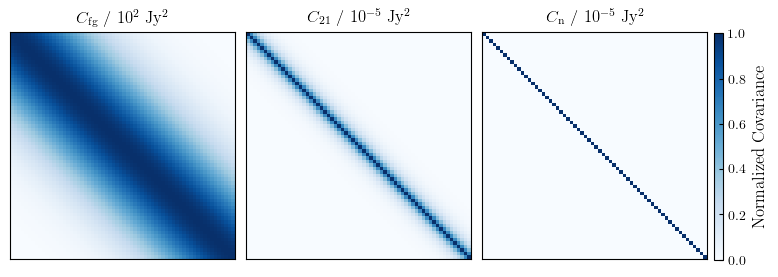
\includegraphics[scale=0.8]{imgs/data_covariance.png}
\caption{The covariance of the foregrounds, EoR, and noise components of our analytic data simulations.
Parameters for the foreground covariance ($\sigmafg^2=10^2\ {\rm Jy}^2$, $\ellfg=4$ MHz) are selected to be roughly characteristic of HERA data.
The EoR covariance parameters ($\sigmato^2=10^{-5}\ {\rm Jy}^2$, $\ellfg=0.75$ MHz) are selected to be roughly in line with fiducial theoretical expectations \citep{Mertens2018}, and the noise is artificially selected depending on the amount of integration assumed for the data.}
\label{fig:data_covariance}
\end{figure*}

How do we actually compute these quantities?
The $\E_\alpha$ matrix can be decomposed as
\begin{align}
\label{eq:qe_E}
\E_\alpha = \frac{1}{2}\sum_\beta \M_{\alpha\beta} \R^\dagger \C_{,\beta} \R,
\end{align}
where $\M$ is a normalization matrix that ensures the estimated band powers are properly normalized, and $\R$ is an arbitrary data-weighting matrix, both of which the data analyst is free to choose subject only to the constraint that our band powers are properly normalized, or that $\sum_\beta\W_{\alpha\beta}=1$.
Here we also see the main role of $\C_{,\alpha}$ as a Fourier transform operator for the weighted data vectors on either side of it.
Given a choice of $\C_{,\alpha}$ and $\R$, we can form the quantity
\begin{align}
\label{eq:H_mat}
H_{\alpha\beta} = \frac{1}{2}\tr[\R^\dagger\C_{,\alpha}\R\C_{,\beta}],
\end{align}
which conveniently lets us re-express the window functions as
\begin{align}
\label{eq:window_func}
\W = \M \H.
\end{align}

The commonly adopted $\R$ matrix in the literature is $\R = \C^{-1}$, or the inverse data covariance matrix.
Given this weighting matrix and assuming a diagonal normalization matrix of $M_{\alpha\beta} = \delta^k_{\alpha\beta}\left(F_{\alpha\beta}\right)^{-1}$ where $\delta^k$ is the Kronecker delta, it can be shown that we recover the optimal, minimum variance estimator \citep{Tegmark1997}.
In such a limit, we get that $\H = \F$ and $\boldsymbol{\Sigma} = \F^{-1}$, where $\F$ is the band power Fisher matrix \citep{Hamilton1997a, Tegmark1997, Bond2000}.
Alternative choices of the normalization matrix lead to other desirable properties, such as $\M=\H^{-1}$ leading to window functions that are diagonal in $k$ space, and $\M=\H^{-1/2}$ leading to a band power covariance that is uncorrelated between $k$ modes \citep{Tegmark2002}.
While $\M=\H^{-1}$ deconvolves the window function, it does so at the expense of larger errorbars.
We therefore only use the minimum variance normalization (referred to as $\M\propto\I$) and the uncorrelated covariance normalization (referred to as $\M=\H^{-1/2}$) in this work.
Regardless of the chosen normalization matrix, we refer to the optimal quadratic estimator as one that adopts $\R_{\rm OQE} = \C^{-1}$, which is also the ``inverse variance weighted foreground removal estimator'' described in \citet{Liu2011}.

To cast Gaussian process foreground subtraction into the quadratic estimator framework, we recognize that \autoref{eq:res} is simply a linear operation on the data vector, and can be equivalently expressed as
\begin{align}
\label{eq:gprfs}
\r = \d - \Exp[\f^\prime] = (\I - \Kfg[\Kfg + \Kto + \Kn]^{-1})\d  = \R_{\operatorname{GPR-FS}}\d.
\end{align}
A quadratic estimator that enacts a GPR foreground subtraction as part of its weighting matrix (referred to as GPR-FS) is therefore achieved by adopting the above $\R$ matrix.
Furthermore, variations about this technique are possible by dotting this matrix into other subsequent operators, such as additional, post-foreground removal weighting matrices.

\subsection{The Relationship Between GPR-FS and OQE}
\label{sec:gpr_oqe}

Here we show that the GPR foreground subtracted quadratic estimator (GPR-FS) is closely related to the optimal quadratic estimator, and is in fact identical to OQE when dotting the former with an additional inverse covariance weighting matrix.
For the time being, we will assume we know the true covariance of the data and will adopt terms like $\Cfg$ instead of $\Kfg$ in our equations.
We can prove the equivalence of these two estimators by using the Woodbury matrix identity, which states that for an invertible matrix $\A$ and for a matrix $\B$ that can be decomposed as $\B = \U\S\V^\dagger$,
\begin{align}
[\A + \U\S\V^\dagger]^{-1} = \A^{-1} - \A^{-1}\U[\S^{-1} + \V^\dagger\A^{-1}\U]^{-1}\V^\dagger\A^{-1}.
\end{align}
In our case, both $\A$ and $\B$ are taken to be Hermitian covariance matrices, implying that $\U$ and $\V$ are unitary matrices subject to $\U\V^\dagger = \I$, with $\S$ being a diagonal eigenvalue matrix.
Re-arranging, we find that
\begin{align}
[\A + \U\S\V^\dagger]^{-1} &= \A^{-1}(\I - \U[\A\U\S^{-1} + \U]^{-1}) \nonumber \\ 
&=\A^{-1}(\I - \U\S\V^\dagger[\A + \U\S\V^\dagger]^{-1})
\end{align}
where in the first equality we pulled $\V^\dagger\A^{-1}$ into the bracketed inverse and used the fact that $[\V^\dagger]^{-1} = \U$, and in the second equality formed the quantity $\U = \U\S\V^\dagger[\S\V^\dagger]^{-1}$ and pulled part of it into the bracketed inverse.
Substituting in $\A = \Cn + \Cto$ and $\B = \Cfg$, we get that
\begin{align}
[\Cn + \Cto + \Cfg]^{-1} &= [\Cn + \Cto]^{-1}(\I - \Cfg[\Cn + \Cto +  \Cfg]^{-1}) \nonumber \\
\R_{\rm OQE} &= [\Cn + \Cto]^{-1}\R_{\operatorname{GPR-FS}}
\end{align}
which tells us that a GPR-FS weighting matrix dotted with an additional inverse noise and EoR covariance weighting matrix is equal to the inverse of the full data covariance matrix.
Given that the statistical properties of a quadratic estimator are uniquely defined by the choice of $\R$ matrix (holding our choice of $\C_{,\alpha}$ constant), we conclude that the optimal quadratic estimator and the inverse variance weighted GPR-FS estimator are actually identical power spectrum estimators.
This is an interesting and non-intuitive result that helps us understand the properties of both of these methods.
First, we see that the inverse covariance foreground separation method of \citet{Liu2011}--the OQE of the 21\,cm signal in the presence of foregrounds--can in fact be re-cast as a Gaussian Process, with \autoref{eq:fg_conditional} yielding its constrained foreground estimate.
Second, we see that the window function and band power covariance matrices for the GPR foreground subtraction technique can be easily derived, and are in fact similar to those for the optimal estimator.

\begin{figure*}
\centering
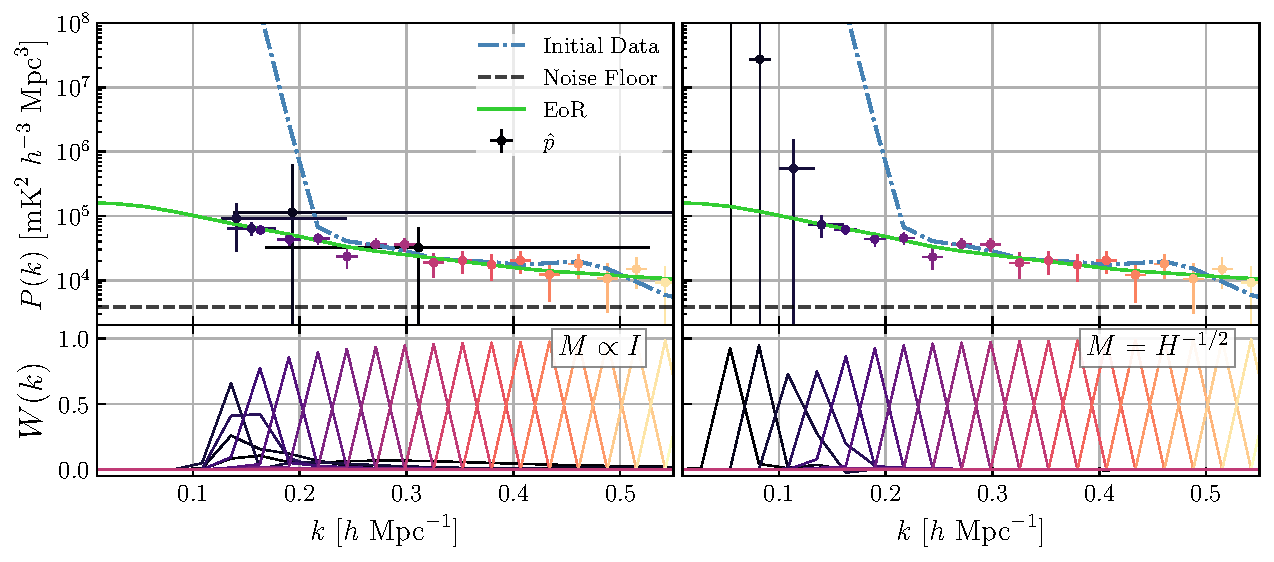
\includegraphics[width=\linewidth]{imgs/gpr_window_low_noise_ell075.pdf}
\caption{Mock GPR foreground separation for two different EoR models ($\ellto$ = 0.25 \& 0.75 MHz) and two different normalization schemes, $M\propto I$ (left) and $M=F^{-1/2}$ (right), in a \emph{low noise scenario} where we get a nominal 10$\sigma$ detection at $k\sim0.2\ h\ {\rm Mpc}^{-1}$.
We show the full data consisting of foregrounds, EoR, and noise (blue dashed), the integrated noise floor of the data (black dashed), the intrinsic EoR component (green solid), and the GPR-FS quadratic estimates (purple dots) after 1000 (independent) incohorent averages.
The error bars on the band powers are their 1$\sigma$ uncertainty ($\sqrt{\Sigma_{\alpha\alpha}}$).
For both EoR models and under both normalization schemes, GPR-FS returns unbiased band power estimates at large $k$ modes.
However, we see that without band power decorrelation (i.e. in the $\M\propto\I$ regime), GPR-FS fails to return statistically independent estimates of the band powers for $k<0.1\ h\ {\rm Mpc}^{-1}$, evidenced by the lack of power in the window functions (lower right).
Although the decorrelated band power window functions demonstrate they can make largely statistically independent measurements at these low $k$ modes, their associated uncertainty is dramatically inflated.}
\label{fig:gpr_window_low_noise}
\end{figure*}

Lastly, we note that GPR foreground subtraction need not only apply to foregrounds.
By simply substituting $\Kfg$ with the sum of any number of (uncorrelated) covariances describing terms in the data that we would like to subtract, we can construct a GPR-based signal separation estimator that is functionally equivalent to what the optimal quadratic estimator would achieve.

\begin{figure*}
\centering
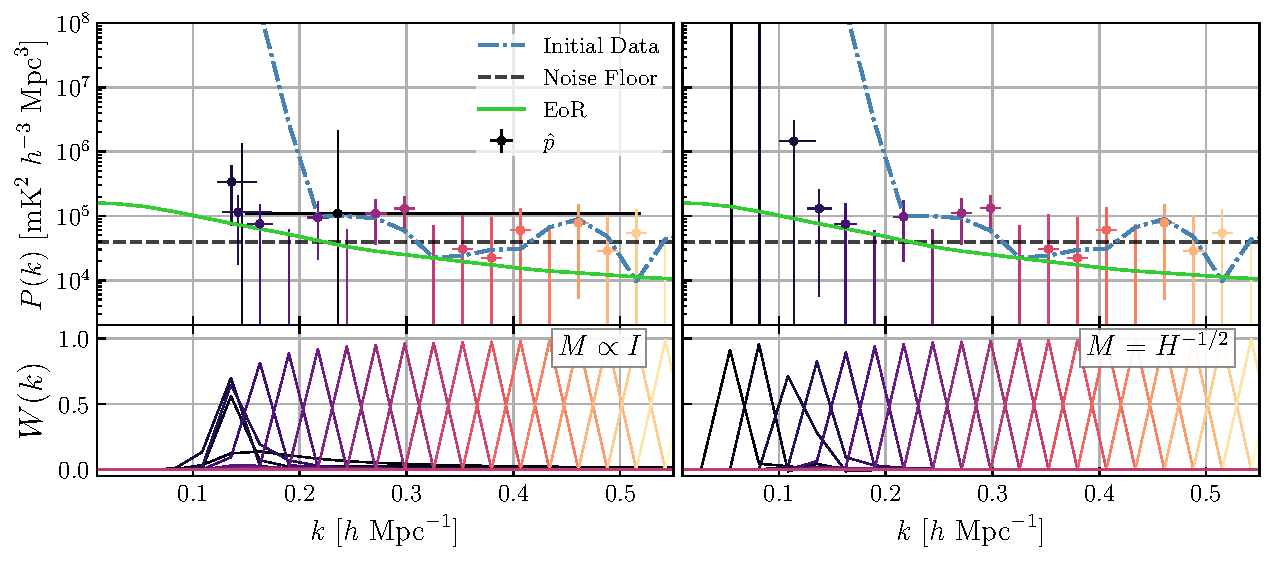
\includegraphics[width=\linewidth]{imgs/gpr_window_med_noise_ell075.pdf}
\caption{The same as \autoref{fig:gpr_window_low_noise} but in a \emph{moderate noise scenario}, where the averaged noise floor roughly meets the EoR signal at $k\sim0.2\ h\ {\rm Mpc}^{-1}$.
In this scenario the window functions are slightly better behaved; however, we still see that GPR-FS with $\M\propto\I$ normalization is unable to probe the very low $k$ modes of the power spectrum (left panel).
While $\M=\H^{-1/2}$ normalization suffers from larger errorbars at low $k$ (right panel), it is able to actually probe these $k$ modes after partially deconvolving the window function.}
\label{fig:gpr_window_med_noise}
\end{figure*}

\subsection{Mapping the Window Functions}
\label{sec:gpr_windows}

One of the blessings of incorporating GPR modeling into the quadratic estimator formalism is the ability to propagate its effect on the band power covariance and window function matrices.
Recall that the window functions tell us how the intrinsic band powers map into our measured band powers.
In a sense, they represent the true $k$ modes that our measured band powers are sensitive to and the width of the band power bin (i.e. the horizontal error bar).

Although in this section our data model extends only to a single baseline (and thus a single $\kperp$ mode), we can still spherically average the band powers from a $\bk$ vector space onto a $|\bk|$ space: in other words averaging Fourier modes of equal magnitude but opposite sign.
Assuming the mapping between the band powers of the true spherical power spectrum to the discretized band powers of the estimated cylindrical power spectrum can be described by a design matrix and an error term,
\begin{align}
\hat{\p}_{\rm cyl} = \A\p_{\rm sph} + \boldsymbol{\epsilon},
\end{align}
then the optimal compression of the cylindrical band powers onto a spherical basis \citep{Dillon2014} is given as
\begin{align}
\hat{\p}_{\rm sph} = \left[\A^T\bSigma_{\rm cyl}^{-1}\A\right]^{-1}\A^T\bSigma_{\rm cyl}^{-1}\hat{\p}_{\rm cyl},
\end{align}
with a covariance matrix
\begin{align}
\bSigma_{\rm sph} = \left[\A^T\bSigma_{\rm cyl}\A\right]^{-1}
\end{align}
and a window function matrix
\begin{align}
\label{eq:sph_window}
\W_{\rm sph} = \left[\A^T\bSigma_{\rm cyl}^{-1}\A\right]^{-1}\A^T\bSigma_{\rm cyl}^{-1}\W_{\rm cyl}\A.
\end{align}
For each estimated band power, $\hat{p}_\alpha$, its vertical error bar is given as $\sqrt{\Sigma_{\alpha\alpha}}$, even though there may be non-zero off-diagonal components for the $\alpha$ band power.
If we regard the window function as a probability distribution, we can estimate the central Fourier bin of the band power, $\hat{k}_\alpha$, as the window function's 50th percentile.
The difference between this estimate, $\hat{k}$, and the $k$ mode we would have naively measured with a simple ``Fourier transform and square'' estimator is one of the key takeaways from this section.
Furthermore, the horizontal errorbars of the band power can be estimated as the window function's 16th and 84th percentile, or its 68\% confidence interval in the Gaussian limit.

To demonstrate an idealized case of GPR-FS and to map its window functions, we generate mock visibility data from the foreground, EoR, and noise covariances described in \autoref{sec:gpr}.
\autoref{fig:data_covariance} shows the covariances of our three data terms.
Again, we assume that we know the true covariance of the data a priori (relaxation of this assumption is deferred to future work).
We simulate the visibility for a single baseline spanning 20 MHz of bandwidth in 64 frequency channels by drawing from a mean--zero complex Gaussian distribution with the covariances described above for each of the foreground, EoR, and noise terms, before summing them together to form our data vector $d$.
For power spectrum estimation, we form two quantities, $\d_1 = \f + \e + \n_1$ and $\d_2 = \f + \e + \n_2$, which have the \emph{same} foreground and EoR realization but independent noise realizations.
These terms enter the left-hand and right-hand side of \autoref{eq:qe} such that our final power spectra are free of the noise-bias component of $b_\alpha$, a common analysis technique performed on real data.
We repeat this 1000 times (drawing an independent realization of all terms each time) and stack them to construct a data vector $\d$ of shape $(N_{\rm freqs}, N_{\rm realizations}) = (64, 1000)$.
Because this uses the same covariance for each draw, one can think of this as drawing over a combination of different baseline orientations (of similar length) and patches of the sky, which will help average down sample variance of the signal terms in the estimated power spectrum.
Technically, we anchor this bandwidth at 150 MHz (for a 140 -- 160 MHz spectral window), but this is effectively inconsequential to this work, as the covariances are fixed:
the only impact this has is on the overall cosmological normalization (i.e. the prefactors in \autoref{eq:dspec}).

We simulate two scenarios that may be relevant over the next few years for 21\,cm experiments: one where the EoR signal is detected at high significance with a signal-to-noise ratio (SNR) > 10 (low-noise scenario) and another where the EoR is marginally detected with SNR = 1 (moderate noise scenario).
The low-noise scenario is shown in \autoref{fig:gpr_window_low_noise}, where the two panels show the measured power spectra with $\M\propto\I$ normalization (left) and $\M=\H^{-1/2}$ normalization (right). The intrinsic EoR signal is overlaid (green), as well as the thermal noise floor after averaging.


\begin{figure}
\centering
\includegraphics[scale=0.6]{imgs/wideband_gpr_Q}
\caption{A schematic of the wideband GPR response matrix $\C_{,\alpha}^{\rm wide}$, which has as a subset of its entires the same response matrix $\C_{,\alpha}$ as before.
Although $\C^{\rm wide}_{,\alpha}$ is dotted into the full wideband data vector after GPR foreground removal, it only estimates band powers over the same narrower bandwidth used previously.}
\label{fig:wideband_gpr_Q}
\end{figure}

\begin{figure}
\centering
\includegraphics[scale=0.6]{imgs/wideband_gprfs}
\caption{GPR-FS applied to a 140 -- 160 MHz bandwidth (left) and wideband GPR-FS applied to a 120 -- 180 MHz bandwidth but with a power spectrum spectral window of 140 -- 160 MHz (right).
Both power spectra are normalized with $\M=\H^{-1/2}$.
As before, we show the full dataset (blue dashed), the EoR component (green) and thermal noise floor (black dashed).
With wideband GPR-FS, we can probe the power spectrum down to lower $k$ with less uncertainty.
However, with this data model, measuring the band powers for $k < 0.1\ h\ {\rm Mpc}^{-1}$ is still challenging.}
\label{fig:wideband_gprfs}
\end{figure}


\subsection{Wideband GPR-FS}
\label{sec:wideband_gpr}

In this section we propose a method for modeling and removing foregrounds across a wide frequency bandwidth (thus achieving finer delay resolution in Fourier space), while simultaneously taking narrow-band power spectra.
The advantage to this, as opposed to modeling the foregrounds over the same narrower bandwidth used for estimating the power spectrum, is the improved behavior of the resultant window functions, driven by the finer delay resolution achievable when modeling across a wider bandwidth \citep{Parsons2014}.
This comes at the cost of increased computational complexity (recall GP's naively scale as $N^3$) as well as an increased data model complexity.
Previous works applying GPR foreground subtraction have made simplifying assumptions driven in part by the adoption of a narrow bandwidth--namely that the foreground and noise covariance amplitude is constant over the band.
Over wide bandwidths, this assumptions breaks down, as both the foreground and noise variance increase significantly with decreasing frequency: in practice, an amplitude power law model would need to be added to the foreground and noise covariances.
In this section we do not actually do this, as this is merely a proposal for how one can setup a wideband GPR-FS matrix, and is meant to demonstrate the improved performance over a narrowband GPR-FS (a similar test for a visibility filtering matrix is done in \citet{Ewall-Wice2020}).


%A wideband GPR-FS is simply a larger, rectangular $\R$ matrix of shape $N_{\rm spw\ freqs}\times N_{\rm freqs}$, where $N_{\rm spw\ freqs}$ is the number of frequency channels in the narrowband spectral window used for power spectrum analysis, and $N_{\rm freqs}$ is the number of frequencies across the wider bandwidth used for GPR modeling.
To demonstrate this, we use the same analytic covariances from before, but inflate them to a size of $196\times196$ frequency channels spanning 120 -- 180 MHz (tripling the bandwidth).
We also construct a larger $196196$ GPR-FS matrix to perform the wideband foreground subtraction.
The key to retaining the same narrow bandwidth for power spectrum estimation comes from a new $\C_{,\alpha}^{\rm wide}$ matrix, which is zero for all entries except for a block along the diagonal located at the desired spectral window for power spectrum estimation, which is populated with the same $\C_{,\alpha}$ from before (\autoref{fig:wideband_gpr_Q}).



\begin{figure}
\centering
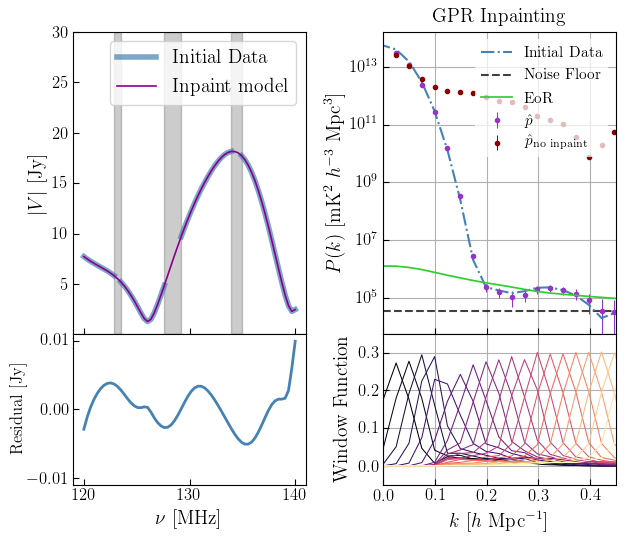
\includegraphics[scale=0.5]{imgs/gpr_low_noise_inpainting}
\caption{GPR inpainting applied to the mock dataset from above. {\bfseries Left}: We show the initial data (blue) with flags applied (shaded) and the inpaint model (purple), which is only summed with the data in the flagged regions. The residual between the inpaint model and the initial data is also plotted (bottom). {\bfseries Right}: We plot the inpainted power spectrum compared to the original data (purple), EoR signal (green solid) and the noise floor (black dashed), along with the non-inpainted band powers (red). All power spectra are normalized with $\M\propto\I$ convention. We also show the inpainted window functions (bottom). }
\label{fig:gpr_low_noise_inpainting}
\end{figure}

\subsection{Inpainting Missing Data}
\label{sec:inpainting}
Often when working with real instruments we must excise or flag data due to poor quality.
This can motivated by detector or instrument failures or by contamination of certain parts of the data, for example due to radio frequency interference.
Intensity mapped power spectra are particularly sensitive to missing data along the frequency axis, as a Fourier transform of discontinuous features will cause ringing of bright Fourier modes (such as foregrounds) to other modes thus contaminating them.
Solutions to this problem have been to remove as much of the foregrounds as possible in the frequency domain (see \citet{Ewall-Wice2020} for an example of this), or to deconvolve the effect of missing data in Fourier space.
Nevertheless, for realistic foreground subtraction techniques we often find residual systematic features that are stronger than the EoR signal in certain parts of Fourier space.
In theory, band power decorrelation (e.g. setting $\M=\F^{-1}$) can help with this, but the impact of missing data can often lead to ill-conditioned matrices in the quadratic estimator. (\nsk{this is just my intuition having trouble doing so in practice}).
Inpainting can help prevent these features from contaminating other modes in the first place.
In practice we are less concerned about the EoR signal ringing against itself in Fourier space, as most theoretical models predict fairly flat features in $P(k)$, but in general this is still a concern, and eliminating the ringing of the EoR signal can help to prevent unnecessary correlation between nearby band powers of high SNR detections.
Furthermore, another reason for wanting to inpaint the data is because we often want to make power spectra of the foreground component, as this is a useful metric for assessing data quality and performing jacknife and null tests.

In general, the problem of reconstructing a signal from incompletely sampled data is known as compressed sensing.
An example of a well-known radio astronomy technique for solving this problem is the Hogbom CLEAN algorithm and its derivatives \citep{Hogbom1974}.
A 1D variation of this algorithm applied along the frequency axis of radio visibilities has been extensively used in PAPER and HERA data analyses \citep{Parsons2009, Ali2015, Kerrigan2018, Kern2020a}.
Recently, \citet{Trott2020} explored how GPR inpainting (aka `kriging') can be used to partially mitigate the effect of regularly contaminated frequency bins in MWA data.
In addition, \citet{Ewall-Wice2020} recently presented a linear filter that uses a delay-space maximum likelihood method for inpainting missing data.
Inpainting also has a long history in CMB analyses, applied to both $C_\ell$ estimation () and map making ().
Here we demonstrate how data inpainting can be seamlessly incorporated into the GPR-FS quadratic estimator, thereby including its effect into the full statistical description of the band power window function and covariance matrix.

Recall \autoref{eq:gp_conditional} gives the distribution of the desired latent variable conditioned on the data.
For the purposes of foreground subtraction, the desired latent variable was assumed to be the foreground component sampled at the same frequencies as the data (\autoref{eq:fg_conditional}).
For the purpose of inpainting we can relax some of these assumptions.
First, inpainting should only impact the data voxels with missing data, and should not alter otherwise cleanly sampled data.
Therefore, the output of the GP model should be summed with the data vector only at the flagged frequency bins.
Furthermore, we do not want the GP conditioned on the missing data, as it is not part of the statistical distribution we are trying to model.
We can handle this by either giving those frequency bins an infinite noise variance (thus in practice eliminating their contribution to the data model), or we can simply truncate them from the data vector $\d$, as the GP need not sample the data at regularly spaced intervals.
To be consistent with $\nu$ representing the native data frequencies and the input frequencies to the GP, we will adopt the former convention.
Second, we may want to inpaint multiple components of the data, not just the foreground signal.
To capture this, we define $\dip$ as the latent variable to-be-inpainted in frequency space, and $\Kip$ as our model for its covariance.


This leads us to construct a generic Gaussian process data model matrix (GPR-DM)
\begin{align}
\label{eq:gpfm}
\R_{\operatorname{GPR-DM}} = \Kip[\Kfg + \Kto + \Kn]^{-1},
\end{align}
which gives us the GPR estimate of our latent variable at all data frequencies.
We can combine this with the appropriate weighting matrices to construct an inpainting matrix,
\begin{align}
\label{eq:gprip}
\R_{\operatorname{GPR-IP}} = \W_{\rm uf} + \W_{\rm f} \R_{\operatorname{GPR-DM}}
\end{align}
where $\W_{\rm f}$ is a diagonal weight matrix that is zero at unflagged frequencies and one at flagged frequencies, and $\W_{\rm uf}$ is a diagonal weight matrix that is zero at flagged frequencies and one at unflagged frequencies.
When forming power spectra of data with a large dynamic range between Fourier modes, it is often beneficial to apply a tapering function that smoothly connects that data to zero at the band edges (also known as apodization), which limits the Fourier space ringing induced by the fact that our data are finitely sampled.
We can do this adopting $\T\R_{\operatorname{GPR-IP}}$ as our weighting matrix, where $\T$ is a diagonal matrix with a tapering function applied to its diagonal.
A commonly adopted taper--and the one we adopt here--is the Blackman-Harris function, which returns 5 orders of magnitude in sidelobe suppression \citep{Blackman1958}.

In \autoref{fig:gpr_low_noise_inpainting}, we show an example of this estimator applied to the same data products discussed above.
The left panel shows the foreground model constructed from $\R_{\operatorname{GPR-DM}}$ (purple) compared to the initial data, along with the flagged regions (shaded).
The right panels shows the estimated power spectrum with and without inpainting (with $\M\propto\I$ normalization) along with the inpainted band power window functions.
Inpainting helps us recover accurate estimates of the foreground power over spectral windows with missing data, which can be useful for data quality management and null testing of data analysis pipelines \citep{Kolopanis2019}.


%%%%%%%%%%%%%%%%%%%%%%%%%%
%%%%%%%%%% Discussion  %%%%%%%%%
%%%%%%%%%%%%%%%%%%%%%%%%%%

\section{Discussion}
\label{sec:discussion}

\subsection{The Impact of Imperfect Covariance Models}
\label{sec:cov_models}

The results of this section have thus far made the generally unrealistic assumption that we know the true covariance of the data a priori.
In principle this is reconcilable, as we can either estimate the covariance from the data, or adopt a prior covariance, produce power spectra, update the covariance, and iterate \citep{Bunn1995, Tegmark, Padmanabhan2001}.
Empirical covariance estimators have both been studied and used in 21\,cm analyses \citep{Dillon2014, Ali2015, Switzer, Eastwood, Masui}, but have also been a point of contention in the literature, as certain aspects of how one derives and regularizes an empirical covariance have been shown to be susceptible to signal loss \citep{Cheng2018}.
In particular, signal loss was shown to occur when one's covariance is too finely tuned to the dataset at hand: in other words, if the covariance is overfit.
However, another source of concern for foreground subtraction techniques is in the subtraction of the \emph{foreground bias}, $b^{\rm fg}_\alpha = \tr[\Cfg\E_\alpha]$.

In this section, we present a sensitivity analysis of the derived 21\,cm band powers after foreground removal on the relative accuracy of the foreground and 21\,cm covariance matrices.



\subsection{Reconciling the Bias Correction of M20}
\label{sec:bias_correction}

In \citetalias{Mertens2020} Sec. 3.3.2 it is postulated that the inferred variance of the residual vector after GPR foreground subtraction is a biased estimate (biased low), and can be corrected to be unbiased by summing its variance with the variance of the GP foreground estimate (\autoref{eq:fg_cov_conditional}).
In this section, we seek to understand the statistical implications this has on the quoted band powers (particularly at low $k$ modes), and compare it to the $\M$ matrix normalization step of the quadratic estimator.

First, we will define the relationship between the unnormalized band powers, $\hat{\q}$, and the normalized band powers, $\hat{\p}$, within the quadratic estimator framework.
We can define the unnormalized band powers as
\begin{align}
\label{eq:unnorm_q}
\hat{q}_\alpha = \frac{1}{2}\d^\dagger\R^\dagger\C_{,\alpha}\R\d,
\end{align}
such that the final normalized band powers can be succinctly expressed as
\begin{align}
\hat{p}_\alpha = \sum_\beta M_{\alpha\beta}\hat{q}_\beta - b_\alpha.
\end{align}
If we assume that our $\M$ matrix is diagonal ($\M\propto\I$), then this final equality simplifies to $\hat{p}_{\alpha} = \sum_\alpha M_{\alpha\alpha}\hat{p}_\alpha - b_\alpha$.
Here we see the quantity $\hat{q}_\alpha$ as simply the weighted and Fourier transformed data vector, while the matrix $\M$ is a multiplicative factor that ensures the final band powers are properly normalized.


Next, to summarize \citetalias{Mertens2020}, the covariance of the residual vector after GPR foreground removal can be shown to be
\begin{align}
\label{eq:res_covariance}
\langle\r\r^\dagger\rangle &= \R_{\operatorname{GPR-FS}}\langle\d\d^\dagger\rangle\R_{\operatorname{GPR-FS}}^\dagger \nonumber \\
&= [\Cn + \Cto] - \Cfg + \Cfg[\Cfg + \Cn + \Cto]^{-1}\Cfg \nonumber \\
&= \C_{\rm r} - \Cov[\f],
\end{align}
where we made the key assumption that our covariance models (i.e. $\Kfg$, etc) are equal to the true covariance of the data (i.e. $\Cfg$, etc).
This tells us that in order to unbias our covariance estimator, we should sum it with the covariance of the GPR foreground estimate.
We can equivalently frame this in terms of the power spectrum by noting that
\begin{align}
\langle\r\r^\dagger\rangle\C_{,\alpha} &= [\C_{\rm r} - \Cov[\f]]\C_{,\alpha} \nonumber \\
2\langle\hat{q}_\alpha\rangle &= \tr[\C_{\rm r}\C_{,\alpha}] - \tr[\Cov[\f]\C_{,\alpha}],
\end{align}
where in the second equality we used the fact that $\tr[\langle\r\r^\dagger\rangle]\C_{,\alpha} = \langle\tr[\r^\dagger\C_{,\alpha}\r]\rangle$.
Thus, assuming a diagonal $\M$ normalization matrix, we can form the quantity
\begin{align}
\langle\hat{p}_\alpha\rangle = \sum_\alpha M_{\alpha\alpha}\langle\hat{q}_\alpha\rangle
\end{align}



\begin{figure*}
\centering
\includegraphics[scale=0.8]{imgs/lofar_shifted_limits}
\caption{LOFAR upper limits on the 21\,cm power spectrum at $z=9.1$ from \citetalias{Mertens2020} assuming the central $k$ bin of each band power is i) the naive discrete Fourier transform (DFT) $k$ bins (filled markers) and ii) using the band power window function 50th percentile (open markers).
The window functions are computed given their adopted data covariances used for GPR foreground removal.
Because the quoted power spectra are in units of $\Delta^2 = P(k) k^3/(2\pi^2)$, adopting different $k$ bin values for the band powers can dramatically change the sensitivity of the limits.
If the window functions computed here are similar to the true LOFAR window functions in \citetalias{Mertens2020}, they call into question the constraining power of the lowest $k$ modes in the quoted power spectrum limit.
This is particularly important for astrophysical parameter space searches for as which are generally the most sensitive $k$ modes and for astrophysical parameter space searches \citep{Ghara2020}, will domin
}
\label{fig:lofar_shifted_limits}
\end{figure*}

\subsection{Implications for Previous Upper Limits}

Here we perform a rough estimate of the implications of un-normalized GPR foreground removal on the band power window functions from the recent LOFAR upper limit of \citetalias{Mertens2020}.
Because \citetalias{Mertens2020} form power spectra from the GPR-FS residuals without decorrelating the band powers and apply a per-band power normalization (as discussed above), the resultant window functions will be similar to the $\M\propto\I$ QE window functions presented in this work.
We construct the $\R_{\operatorname{GPR-FS}}$ matrix used in the LOFAR analysis from the five covariance terms of their GPR model and their hyperparamter values from their Table X.
We model the data covariance from XXX -- XXX MHz with 64 channels, which are then averaged onto the X number of logarithmic $k$ bins in the process of spherical averaging, using \autoref{eq:sph_window} to compute the window functions for each band power.



%%%%%%%%%%%%%%%%%%%%%%%%%%%%%%%%%%%%%%%%%%
%%%%%%%%%%%%%%%%% Conclusion %%%%%%%%%%%%%%%%%%%
%%%%%%%%%%%%%%%%%%%%%%%%%%%%%%%%%%%%%%%%%%
\section{Conclusions}
\label{sec:conclusions}

In this work we have investigated Gaussian process regression for foreground subtraction in 21\,cm surveys of the EoR.

One of the key assumptions we made for GPR and QE foreground subtraction in \autoref{sec:gprfs} was the equivalence between the adopted data covariance matrix and the true, underlying covariance matrix.
One can empirically estimate this directly from the data \citep[e.g.][]{Dillon2014}, but this has also been shown to cause signal loss if not handled properly \citep{Switzer2016, Cheng2018}.
Future work will study the impact of real-world covariance model imperfections on GPR and QE-based foreground separation.


\section*{Acknowledgements}

%We would like to thank Florent Mertens, Abhik Gosh, Gianni Bernardi and ... for feedback on a draft of this manuscript.




%%%%%%%%%%%%%%%%%%%%%%%%%%%%%%%%%%%%%%%%%%%%%%%%%%

%%%%%%%%%%%%%%%%%%%% REFERENCES %%%%%%%%%%%%%%%%%%

% The best way to enter references is to use BibTeX:

\bibliographystyle{mnras}
\bibliography{eor_references} % if your bibtex file is called example.bib


%%%%%%%%%%%%%%%%%%%%%%%%%%%%%%%%%%%%%%%%%%%%%%%%%%

%%%%%%%%%%%%%%%%% APPENDICES %%%%%%%%%%%%%%%%%%%%%

\appendix

\section{Computational Complexity}
Naive scaling of $N^3$, optimized scaling of $N^2$ for low and intermediate $N$.




%%%%%%%%%%%%%%%%%%%%%%%%%%%%%%%%%%%%%%%%%%%%%%%%%%


% Don't change these lines
\bsp	% typesetting comment
\label{lastpage}
\end{document}

% End of mnras_template.tex